\documentclass[letterpaper, 11pt]{report}
\usepackage{amsmath}
\usepackage{graphicx}
\usepackage{setspace}
\usepackage[top=4cm, bottom = 4cm]{geometry}
\usepackage{hyperref}
\hypersetup{ linktoc=all }
\usepackage[nottoc]{tocbibind}
\usepackage{appendix}


\begin{document}

\begin{titlepage}
\begin{center}

\begin{spacing}{1.5}
\textbf{PHYS 4909 Honours Project: Final Report}\\
\vspace*{\fill}
\end{spacing}
\begin{spacing}{2.0}
\textbf{\huge Development of an Environmental Monitoring System for the Testing of ATLAS-ITk Microstrip Sensors}\\[0.5cm]
\vspace*{\fill}
\end{spacing}

\begin{spacing}{1.5}
\textit{Submitted by:}

\textbf{\large Keegan Osler}

\vspace*{\fill}
\textit{Supervisor:}

\textnormal{\large Dr. Thomas Koffas}

\vspace*{\fill}

\textnormal{\large CU-ITk Research Team \\ Carleton University Department of Physics \\ Fall 2017/Winter 2018}

\end{spacing}
\end{center}
\end{titlepage}

\pagenumbering{roman}

\begin{abstract}
\addcontentsline{toc}{chapter}{Abstract}
The ITk (Inner Tracking detector) is an upgrade to the innermost part of the detector involved in the ATLAS experiment at the HL-LHC.  It is solid-state powered unlike its predecessor, the motivation for which is the increased luminosity goals of the HL-LHC, as well as other requirements set out by the HL-LHC that the current detectors do not satisfy.  Carleton University's role in this upgrade project involves careful electrical characterization and quality control of the detectors prior to the assembly of the detector modules.

The ITk is composed of two different types of detectors: silicon microstrip detectors and pixel detectors.  The strip detectors are currently being tested at Carleton University before their eventual send off to CERN and are extremely sensitive to changes in the temeprature and humidity of their testing environment.  For this reason, an environmental monitoring system is necessary for the logging and observation of these conditions in the lab.  In this work the development and implementation of such a system will be discussed in detail.
\end{abstract}

\renewcommand{\abstractname}{Acknowledgements}
\begin{abstract}
\addcontentsline{toc}{chapter}{Acknowledgements}

I would first and foremost like to thank my supervisor, Dr. Thomas Koffas, for his guidance and education throughout the course of this project as well as the opportunity to participate in this important physics research for my undergraduate honours thesis.

I would also like to thank the other members of the CU-ITk research team for their assistance with this project, especially James Botte, whose programming and electronics knowledge was absolutely crucial to the ultimate success of the PhysPi. Additionally I would like to acknowledge as well the various faculty and staff at Carleton University for their assistance in acquiring the materials and space for the development of this project.

Lastly I would like to thank the Carleton University Physics Department as well as my classmates, friends, roommates, sister and parents for making it possible for me to be here in the first place.

\end{abstract}

\pagenumbering{arabic}
\tableofcontents
%\newpage
%\pagenumbering{arabic}

\chapter{The LHC and the High Luminosity Upgrade}

CERN's Large Hadron Collider (LHC) is the world's largest and most powerful particle accelerator.  Since 2008 it has been the foremost site for experimental particle physics on earth and is the most complex experimental facility to have ever been constructed.  Sitting below ground under a lightly populated area along the France-Switzerland border near the city of Geneva, the LHC consists of a 27km ring composed of superconducting magnets and also involves many accelerating structures that boost the energy carried by particles travelling through the accelerator.  Along the ring there exist seven detectors which each serve an individual purpose in terms of physics research and each strive to acheive unique goals, all of which ultimately come together to help us understand the nature of our universe and the matter that makes it up.  The goal of the hundreds of physicists around the world that are working alongside the LHC with CERN is to answer open questions in physics concerning aspects of the Standard Model and elementary objects.

\section{The Future: Higher Luminosity}

In July 2012 the LHC achieved it's most significant milestone to date, that being the monumental discovery of the Higgs Boson following decades of development of the theoretical framework which hypothesizes the existence of this particle.  Following this event, a shutdown of the LHC was planned to upgrade and perform maintenence on the many complex and hard-working parts of the collider.  It was then that the "high luminosity" upgrade to the LHC (HL-LHC) was planned for the collider.  Due to several years of running and experimental proceedings, the LHC, like any such complex experimental setup, began to experience diminishing returns and later years of experimentation are expected to yield less significant results comparatively to that whent the detector is working in it's prime.  The logical response to this issue is an upgrade to the collision energy of the particles being accelerated which is done by increasing the luminosity targets of the accelerator.

The upgrade will further the luminosity applied to experiment to anywhere from five to seven times what is currently being used and this will hopefully enable experiments to enlarge their data sets by up to an order of magnitude compared to the current LHC baseline capabilities.  With three "long shutdown" (LS) periods consisting of two years each, the upgrade will further the lifetime of the detector past it's original ten-year lifetime by an extra 17 years, extending it's operability and experimental capacity until 2037.

\section{The ATLAS Experiment}

Of the several detectors that sit along the ring composing the LHC there are two large, general-purpose particles detectors which study the Higgs Boson and search for signs of new physics. A Toroidal LHC ApparatuS (ATLAS) is one such detector and is the backbone of the research outlined in this work.  The detector was monumental in the discovery of the Higgs Boson and shares accolades and honours for the discovery with the Compact Muon Solenoid (CMS), which is the other large, general-purpose detector at the LHC.  ATLAS is a largely cylindrical apparatus and weighs in at around 7000 tonnes.  It has physical dimensions of roughly 46m by 25m by 25m, making it the largest detector in particle physics.  It's operation, maintenence and research employs over 3,000 physicists, research scientists, technologists and students from 175 institutions in 38 countries around the world. It's primary goal is to utilize the unprecedented energy available at the LHC and observe the phenoma that occur with highly massive particles and are not observable using lower-energy accelerators.

ATLAS is designed to detect as many different collision and interaction decay products as possible which results in the detector having a somewhat onion-like geometry which extends into a cylinder.  ATLAS implements different detector technologies which are placed at increasing radii from the interaction point at the centre.  Each of these technologies involves different functionalities for particle detection.  At the heart of the detector is an ionizing particle tracker called the Inner Detector (ID).  It is an upgrade to this innermost part of ATLAS which has provided the basis for this honours project work.

Figure 1.1 shows a diagram of the ATLAS detector and it's inner detector as it is currently.

\begin{figure}[h]
\centering
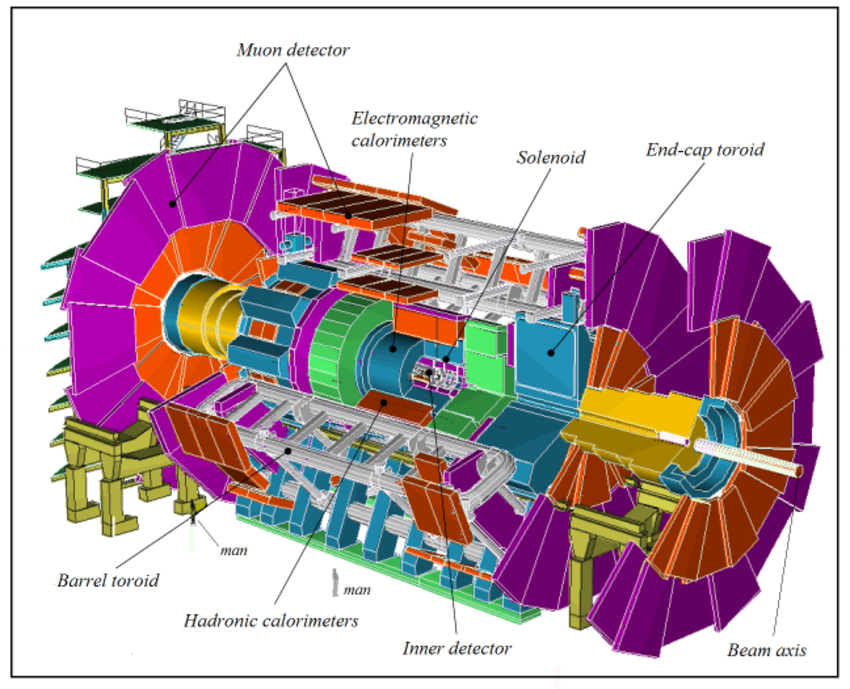
\includegraphics[width=\textwidth]{atlaspres}
\caption{ATLAS Detector Diagram}
\end{figure}

\subsection{ATLAS-ITk Upgrade}

Due to the high luminosity targets being worked towards in the HL-LHC upgrade to the existing LHC, an upgrade to the innermost part of ATLAS is necessary to keep the experimental fully functional and operating at optimal performance under the upcoming changes.  As higher luminosities are reached in the LHC, the ATLAS inner detector will begin to crumble under the higher level of intensity if it maintains current parameters.  Increased luminosity leads to increased detector occupancy as well as increased complexity of collision events.  This in turn leads to increased saturation of the inner detector's capability to collect data from collisions.  As well, as the collision activity is increased over time there will be an increase in damaging effects such as radiation damage and materials activation.  As a result, the ATLAS inner detector will not survive with current parameters and will not be capable of producing accurate results in the HL-LHC.

The solution to this large problem is the Inner Tracker (ITk) upgrade to ATLAS which will replace the ID currently running in conjunction with, and in preparation for, the advancement of the LHC into the higher-luminosity upgrade.  ATLAS-ITk will be a fully solid-state detector revolving around silicon-based technology.  This new construction and materials usage will offer advantages in resolution and radiation hardness, meaning that ITk will be stronger against damaging effects caused by higher luminosity than ID.  To achieve the goals of ATLAS, ITk will utilize this semiconductor material and technology in two different detecting geometries: microstrip and micropixels.  These then compose Strip and Pixel subdetectors which make up ATLAS-ITk.  Research and work related to the development of the silicon microstrip detector system at Carleton University will be the focus of this thesis.

\subsection{ATLAS-ITk at Carleton University}

The CU-ITk team at Carleton University works on the developement and construction of the strip detector system in preparation for it's eventual send off to CERN for implementation.  This involves the careful probing of new sensors and testing of different parameters related to the operation of the detector system, such as it's performance under certain environmental conditions.  Much work is also being done towards the optimization of the strip detector testing environment, which is largely the cleanroom at ME5191 in the university's Department of Electronics (DOE).  This involves the construction of a special probestation for testing of the delicate sensors as well as the development of a simple, accurate and cost-effective environmental monitoring system for the cleanroom.  This system, known as the PhysPi, was designed and implemented by myself as the primary aspect of this thesis and will be covered in detail for the bulk of this report.  

Before the PhysPi can be discussed in detail, it is necessary to outline the underlying semiconductor physics at play in ITk and how this physics contributes to the proposed operation of ITk.  This will be the focus of the next two chapters.

\chapter{Semiconductor Physics}

The basis of the silicon microstrip detectors is the physics of semiconductors.  A semiconductor is material with an electrical conductivity somewhere between that of an insulator and that of a conductor as well as a band gap that exists somewhere between the valence and conduction bands.  This band gap is centered on the Fermi Level, which is defined as the top of the collection of electron energy levels at absolute zero temperature.  This is important to note because electrical conductivity occurs as a result of the presence of electrons in delocalized states, meaning that the state contains an electron only part of the time.  A state is delocalized when it’s energy is near to the Fermi Level.  Thus, in a semiconductor, a finite number of electrons will be able to reach the conduction band and provide a current such that a finite amount of conduction can occur.

In this chapter, fundamental semiconductor physics concepts that are particularly relevant to the ATLAS-ITk silicon microstrip sensors will be discussed.

\section{Doping}

The conducting properties of a semiconductor can be altered via a process known as doping wherein a small concentration of an impurity with a known energy level is introduced into the semiconductor material, adding extra energy levels.  Two types of semiconductors can be formed via doping: p-type semiconductors and n-type semiconductors.  p-type semiconductors are formed when the energy level of the introduced impurity is just above that of the valence band.  In this case, electrons are excited into acceptor levels, leaving behind vacancies or ''holes.''   Conversely, n-type semiconductors are formed when the energy level of the introduced impurity is just below that of the conduction band.  In this case, electrons are excited into donor levels. 

In the case of p-type semiconductors, the majority charge carriers are the holes left behind when the electrons are excited into acceptor levels. These holes will be denoted as h\textsuperscript{+}.   In the case of n-type semiconductors, the majority charge carriers are the electrons themselves.  Electrons will, as usual, be denoted by e\textsuperscript{-}.
\section{The p-n Junction}

A p-n junction is formed when an n-type semiconductor and a p-type semiconductor are brought into contact with each other.  This junction acts as an electrical interface between the two types of materials.

When the n- and p-types are brought together, the two different kinds of majority charge carriers will travel in opposite directions and experience attraction.  This results in the formation of an immobile charged space, since the two sides of the junction are initially electrically neutral.  This charged space will eventually come to equilibrium with the movement of the majority charge carriers and there will then be no mobile charge carriers within the charged space.  At this point, the charged space is referred to as the depletion zone.
\section{Depletion Zone}

Formed as a result of the p-n junction, the depletion zone has many electronically useful characteristics.  The diode nature of a planar p-n junction is exhibited through the resizing of the depletion zone caused by applying a voltage across it.  If this applied voltage acts to counteract the voltage already present in the charged space then the depletion zone will contract.  This is known as forward bias.  Alternatively, if the applied voltage acts to reinforce the voltage already present in the charged space then the depletion zone will expand.  This is known as reverse bias.

Experimentally, it is important and very electronically useful to maximize the size of the depletion zone (i.e., cause reverse bias) as this allows for more charge to be liberated and thus allows for a larger signal to obtained. 


\chapter{ATLAS-ITk Strip Sensors}

An experimental application of the p-n junction and depletion zone physics described in the previous chapter is the ATLAS-ITk microstrip sensor.  This sensor is a large-area \textit{n\textsuperscript{+} - in - p}, AC coupled microstrip, oxygenated float zone (FZ) silicon detector.  Its design and various characteristics pertaining to current experimental work will be described in detail in this chapter.

\section{Overview of ITk Strip Sensors Design}

The aforementioned \textit{n\textsuperscript{+} - in - p} material choice is uncommon and central to the cost effectiveness of the detector as a whole as it nullifies the degrading effects that result from type inversion.  More specifically, this material choice allows for a single sided process as well as operation during partial depletion.  As well, the collection of electrons that occurs via this material choice allows a faster and potentially larger signal to be obtained.

The microstrip detector is composed of a large flat bulk substrate that is of either p- or n-type doping.  On either one or both of the flat sides of this substrate, there are patterned implants of either n or p-type doping (opposite to the doping of the bulk substrate) that extend minimally into the detector in the z-direction relative to the entire width of the bulk substrate.  The mating of these two types results in an array of p-n junctions that are connected in parallel and in reverse bias so as to expand the depletion zone.  Ideally, the depletion zone should expand to cover the entire bulk of the detector.  When this occurs, the electric field present in the detector will be largely vertical and as such any tracking particle will produce a strip-localized cluster from which a position measurement can be obtained.

\section{Characteristics of the ITk Strip Sensors}

There are important physics phenomena applicable to this specific type of detector that must be discussed in depth for an accurate understanding of the detector's operation.

\subsection{Depletion Capacitance}
The depletion capacitance is defined as the capacitance associated with the charge variation that occurs in the depletion zone. 

Given that the implants on the flat side of the bulk substrate extend very minimally in the z-direction, the bulk physics can be approximated as being that of a simple planar p-n junction.  Since the material is initially electrically neutral, there must exist equal space charge on either side of the depletion zone.  It is for this reason that the implants must be of a much higher dopant concentration than that of the bulk substrate; it is required to help further the extent of the depletion zone across the bulk.

In the case of thermal equilibrium, wherein the steady state condition requires that there must exist equal charged spaces on either side of the depletion zone and that the electric field disappears at the boundaries of the zone, a relationship between the depletion depth and the applied reverse bias voltage can be derived.  Since the charged spaces on either side of the depletion zone are immobile, the depletion depth must be inversely proportional to the dopant concentration.  To relate the depletion depth to other necessary parameters, Poisson's equation is invoked and relates the electric potential to the charge distribution present (i.e., the depletion zone).  This results in Equation 2.1 representing depletion depth:

\begin{equation}
d^2 = \frac{2V\epsilon_{sc}}{qN_{eff}}
\end{equation}

Here, \textit{d} denotes the depletion depth, \textit{V} is the reverse bias voltage, \textit{$\epsilon$\textsubscript{sc}} is the dielectric permittivity of the semiconductor material, \textit{q} is the elementary charge(1.602 $\times$ 10\textsuperscript{-19} C) and \textit{N\textsubscript{eff}} is the effective dopant concentration.  In order to achieve optimal sensitivity of the detector (i.e., maximum extension of the depletion zone), a semiconductor with a very high resistivity is required.  The depletion capacitance itself is defined as follows:

\begin{equation}
C = \sqrt{\frac{q\epsilon_{sc}N_{eff}}{2V}}
\end{equation}


In Equation 2.2, \textit{C} represents the depletion capacitance and the remaining quantities are the same as those described for Equation 2.1.  

The depletion volume acts in a similar way to a parallel plate capacitor in that the size of the immobile charge region will be increased with an increase in the applied reverse voltage, thus decreasing the depletion capacitance.

\subsection{Full Depletion Voltage}

The full depletion voltage of the detector is defined as the minimum reverse bias voltage for which the depletion zone will be fully extended; it is the minimum reverse bias voltage for which the detector will perform at optimal sensitivity.  This is an important quantity as it impacts the power consumption of the detector.  As such, it is important to minimize the full depletion voltage as much as possible for optimal power consumption. This can be done by using a high-purity material with tuned doping concentrations.

\subsection{Charge Collection Efficiency}
The charge collection efficiency (CCE) is defined as the ratio of the charge actually captured by the electrode and the total free charge that was initially liberated.  This ratio can be hindered by a phenomenon wherein undesired defects in the material lead to a reduction in the amount of charge that is collected.  In this case, the energy level of the defect in the crystal lattice structure would have to have an energy level within the band gap of the material because a charge carrier that is trapped will then be unlikely to be thermally excited out of that band and into adjacent ones.

A trapping level has a certain depth associated with that energy level's proximity to the material's band gap.  A positive trap that has an energy level near that of the valence level will be deep in depth and will trap electrons, whereas a negative trap with an energy level near that of the valence level will be shallow in depth and will trap the holes instead.

Large traps are created by impurities that are either large in size, such as a defect in the crystal lattice structure of the material, or that are large in terms of charge, such as a chemical impurity.


\subsection{Leakage Current}
Reverse bias leakage current can occur over the depletion zone in the form of reverse current substantiated only by the minority charge carriers h\textsuperscript{+} because the majority charge carriers e\textsuperscript{-} cannot travel across the junction.  This results in a small saturating current in the ideal case.  There are a multiple factors that can contribute to reverse bias leakage current.

One large contributing factor is surface leakage, which occurs over the surface bound depletion zone, that being the space between the bias rail and the edge metal.  The surface leakage has a complex relation to many parameters including the encapsulation, humidity, contamination and edge structure of the detector.

The more dominant factor in the generation of leakage current is the thermal generation of e\textsuperscript{-} and h\textsuperscript{+} pairs that lends to the detector a strong dependence on temperature.  This generation of charge is caused by the presence of impurities in the energy levels which are the aforementioned trapping levels.  The current generated is related to the charge of the specific carrier as well as the depletion zone thickness as this is the volume from which it is generated.  The temperature dependence of this parameter is then brought in when taking into account the generation rate, which is proportional to the number of carriers that are available for promotion as well as the lifetimes of the carriers that are present in the traps.  The concentration of charge carriers in the original semiconductor material is given by Equation 2.3 as follows:

\begin{equation}
n_i (T)     \propto     T^{3/2} e^{\frac{-E_g}{2kT}}
\end{equation}

In this equation, \textit{n\textsubscript{i}} is the concentration with respect to temperature \textit{T}, \textit{k} is the Boltzmann constant (1.38 $\times$ 10\textsuperscript{-23} m\textsuperscript{2} kg s\textsuperscript{-2} K\textsuperscript{-1}) and \textit{E\textsubscript{g}} is the band gap energy.  The temperature dependence of the generation lifetime can be approximated as follows in Equation 2.4 below:

\begin{equation}
\tau_{gen}     \propto    T^{1/2} e^{-\frac{\Delta}{kT}}
\end{equation}

Here, $\tau$\textsubscript{gen} is the generation lifetime, \textit{T} is the temperature, \textit{k} is the Boltzmann constant and $\Delta$ is the difference between the trap energy level and the intrinsic Fermi level.  Assuming that trapping is equally effective for \textsuperscript{-} and h\textsuperscript{+} (which is a reasonable assumption), the generation lifetime can be minimized when the trapping level is closest to the intrinsic Fermi level energy.  Since the mid-gap trap is the one that will generate the majority of the thermal current, the current temperature relation can be approximated by Equation 2.5 where \textit{I\textsubscript{leakage}(T)} is the leakage current with respect to its temperature dependence:

\begin{equation}
I_{leakage}(T)   \propto   T^{2} e^{-\frac{1.21}{kT}}
\end{equation}\\

\chapter{The PhysPi Environmental Monitoring System}

My contribution to the CU-ITk research team and to ATLAS as a whole has been the design, development and implementation of an environmental monitoring system for the cleanroom in which the ITk strip sensor prototypes are tested and probed. This system has been named the PhysPi.  This project took place over the course of the academic year covering September 2017 until April 2018 and is intended to be a tool for use by the CU-ITk team into the future.  Such a system will provide a framework upon which other institutions may create similar systems, and has a wealth of extensions that can be developed by future students.  This chapter will outline in detail the various components of the system as well as how these components were developed to yield the best results in the cleanroom, and how the various steps in the system flow together to monitor temperature and humidity conditions.

\section{PhysPi Overview}

The PhysPi Environmental Monitoring System is a simple, accessible and straightfoward electronic and interface system which consists of a Raspberry Pi 3, an Arduino Uno board, two Sensirion SHT75 sensors, various cables and an immense amount of custom software which involves seven different programming languages (Python, Arduino, bash, MySQL, HTML, PHP and Gnuplot).  As an overview, this system measures the temperature and relative humidity of the air, stores this numerical data in a database for analysis purposes and finally displays plots of this data over time as well as the raw numbers to a user-friendly webpage.  The majority of this is hosted on the Raspberry Pi, hence the name given to the system.

\subsection{Motivation for and Goals of the Environmental Monitoring System}

As was alluded to in the first chapter of this report, the silicon microstrip sensors being tested at Carleton are extremely sensitive to even the slightest changes in the humidity and temperature of the space they are in and thus the results of testing on these sensors are quite easily skewed by changes in temperature or humidity of the air in the cleanroom.  Unfortunately, such disturbances are quite common as the cleanroom is not exclusive to CU-ITk and the space is shared with other research teams within the DOE.  The movement of various people in and out of the room, the turning on and off of fans by university maintenence workers and events within the DOE experiments happening in the same room often cause sudden jumps or drops in the temperature and humidity of the room.  If these incidents are unplanned it can cause undue difficulty in analyzing tests for ITk and slows the pace at which research is completed.  As such, the need for an environmental monitoring system in the cleanroom arose.

It was concluded by the team that such a system would need to have the following attributes:
\begin{itemize}
\item Not embedded within an already existing system that is used for ITk (so that it can still function in the event of ITk equipment failure).
\item Cost effective.
\item Simple and easy to use.
\end{itemize}

At first glance it would seem like the first point on this list negates the other two, but the design produced actually achieves each point.  The Raspberry Pi is a small, single-board computer used often for the teaching of computer science to young people due to it's ease of use and is also used to teach these same skills to people in low-income areas and developing countries due it costing a mere 35USD for just the board.  As the information is displayed on a simple webpage that requires no external manipulation to use this system also achieves the ease of use point listed above.


\section{PhysPi System Hardware}

It is necessary to first outline the physical aspects of the PhysPi, that being the hardware involved in the system.  The hardware is composed of three primary components: sensor technology, Arduino and Raspberry Pi.

\subsection{SHT75 Sensor Technology}

The PhysPi implements two sensors, both of which are the SHT75 by Sensirion.  This is a digital pin-type sensor and is the higher-end version of this Sensirion series.  These sensors are used for many ITK-related tests in the cleanroom and as such were deemed a good fit for this project.

In these sensors a capacitive sensor element measures the relative humidity of the air.  A band-gap sensor measures the temperature of the air.  The SHT75 integrates these sensor elements with signal processing in a compact format to produce a fully calibrated digital output.  Individual calibration of these sensors is not necessary which makes for easy replaceability of the sensors which is a much appreciated feature along with low power consumption.  This unique sensor design allows for optimal thermal coupling to the external environment as well as decoupling from potential sources of heat along the main board.  The SHT75 also provides individual precision calibration, on-chip calibration memory and a digital two-wire interface which all contribute to the easy integration of these sensors into demanding systems and applications.

Figure 4.1 shows the two SHT75 sensors currently being used with the PhysPi before the system was constructed into it's final state.  Much of the development described over the next few sections was performed using only one SHT instead of two for ease and simplicity purposes.

\begin{figure}[h]
\centering
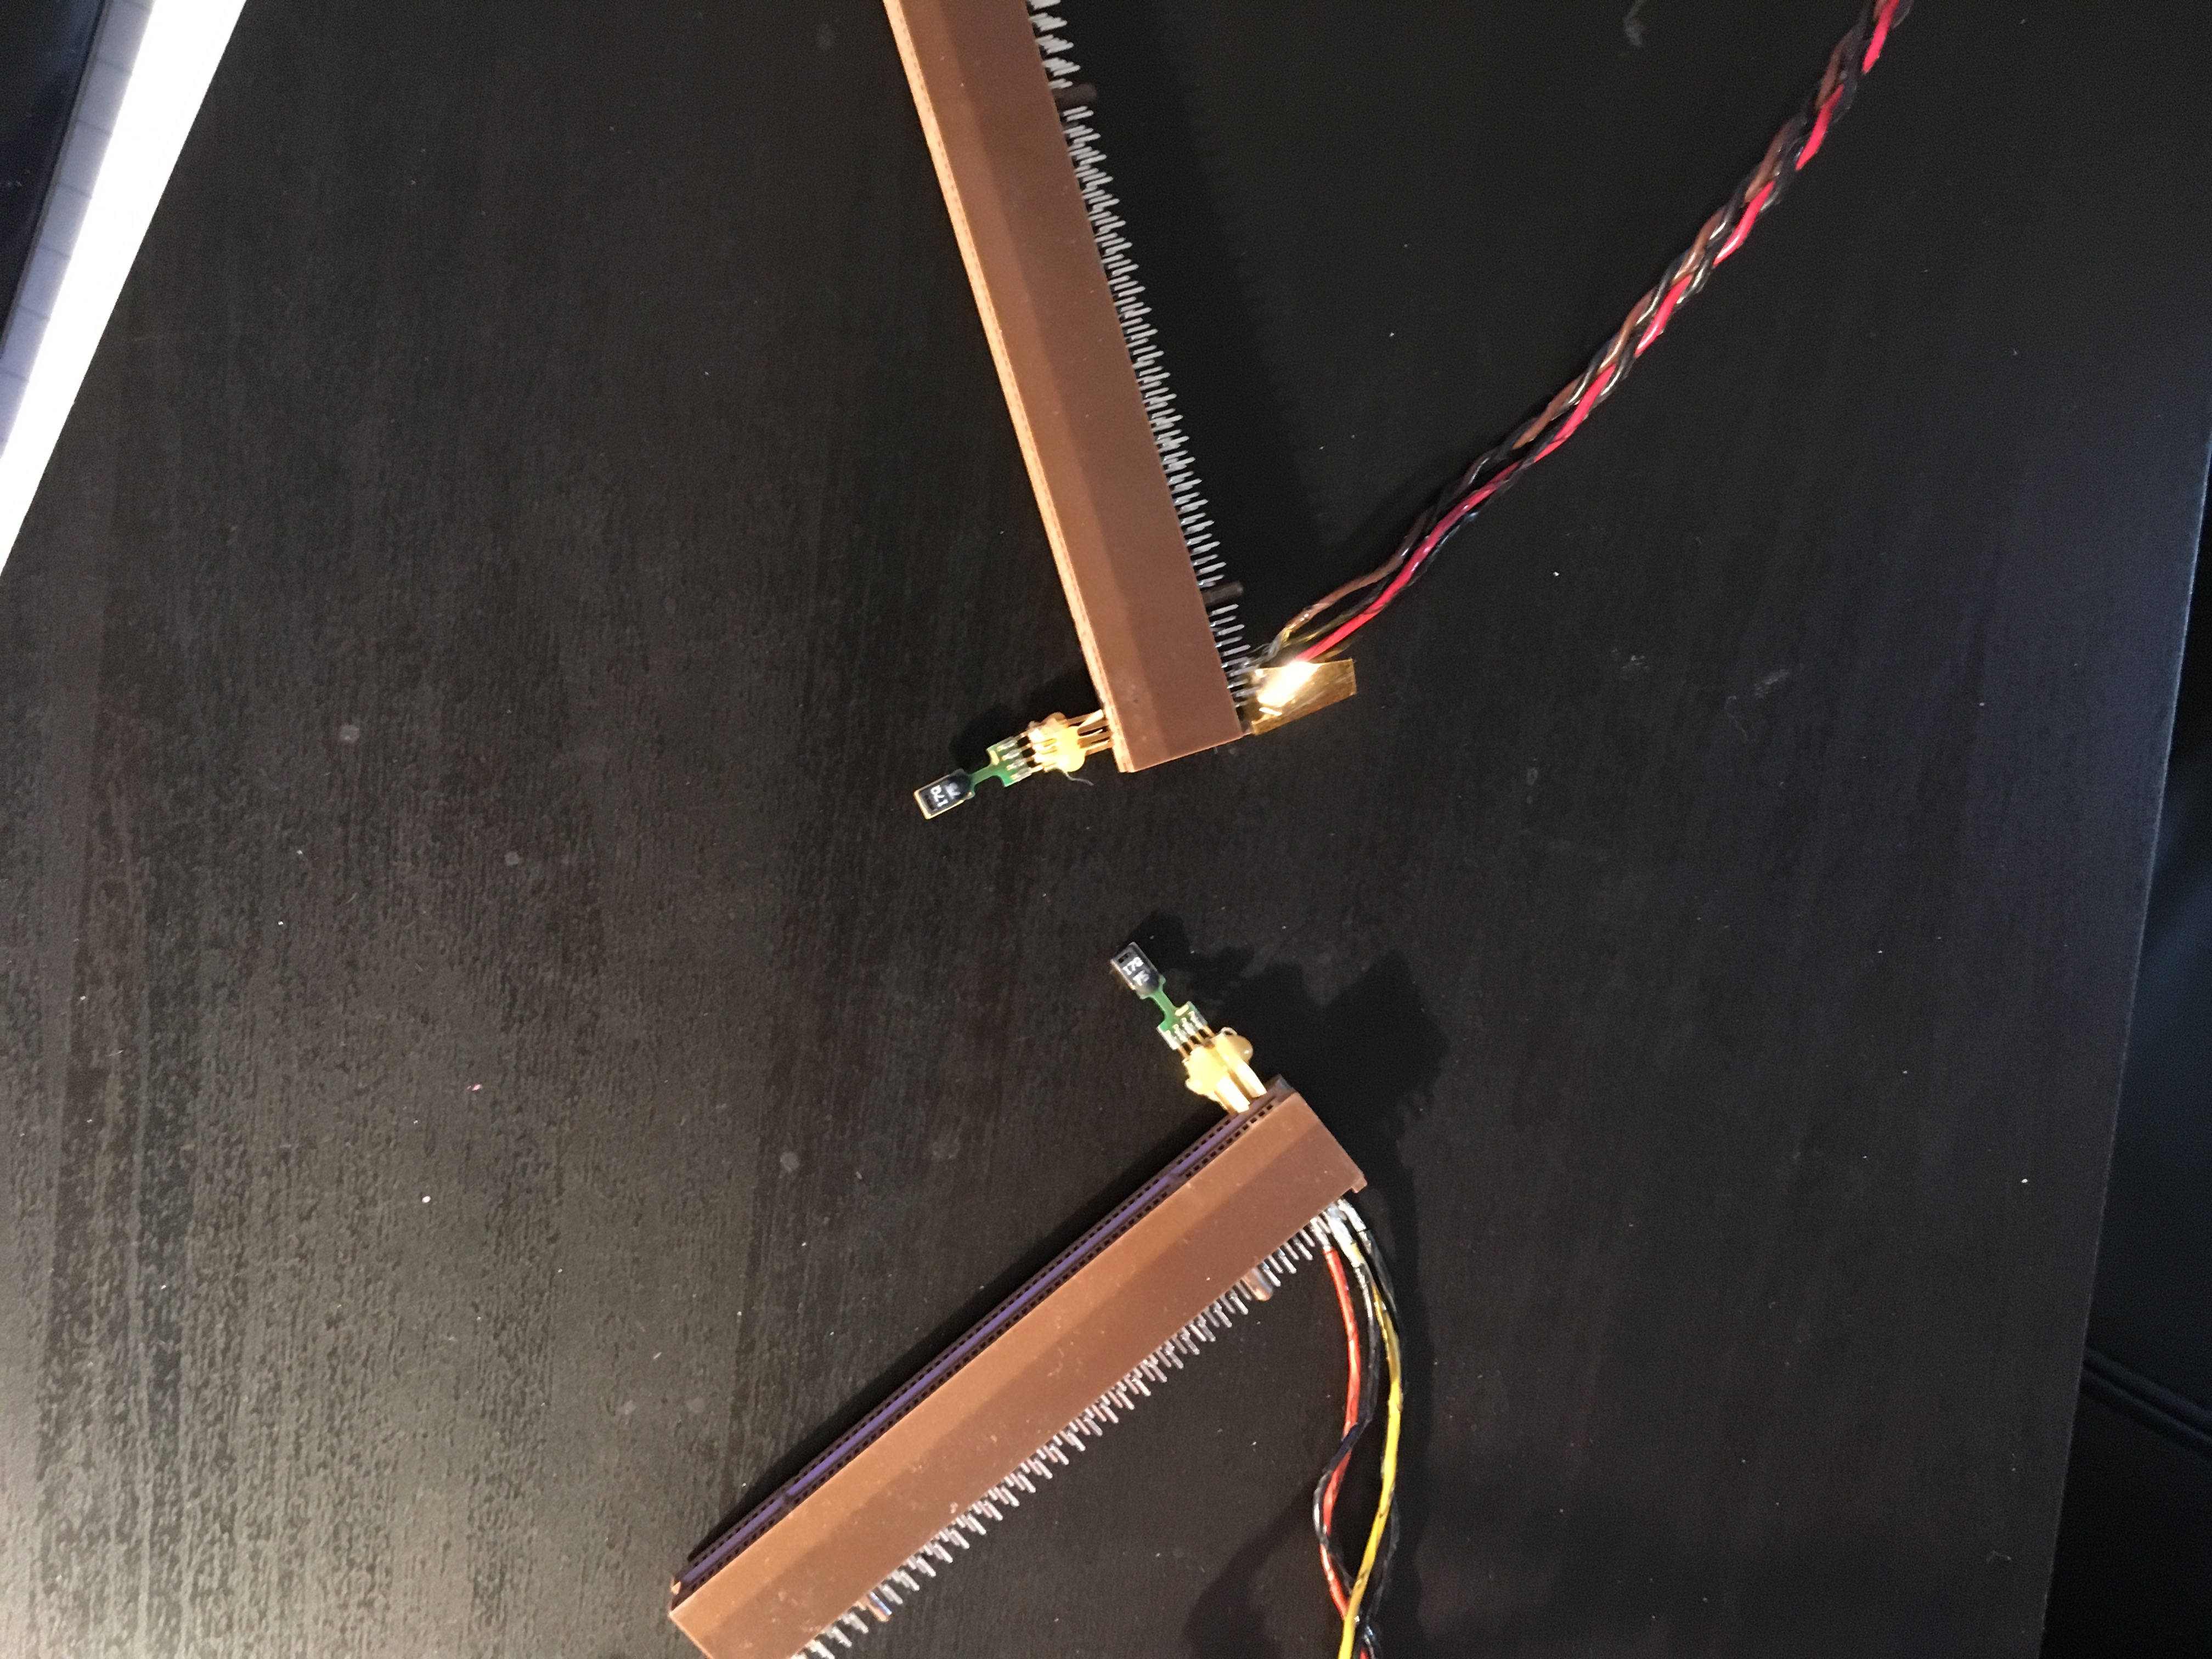
\includegraphics[width=10cm]{2shtrep}
\caption{Sensirion SHT75 Sensors}
\end{figure}

\subsection{Arduino Uno Board}

The SHT75 sensors described in the previous section are wired to an Arduino Uno board in the next step of this process.  Arduino is an open source computer software and hardware company which manufactures single board microcontrollers such as the Arduino Uno board used in the PhysPi. The Uno microcontroller is the most commonly used Arduino board likely due to it's durability and strength which make it the ideal microcontroller for tinkering and experimentation.  This board is used alongside the SHT75 in the cleanroom for many other ITk-related tests.  The board has 14 digital input/output pins, six analog inputs, a 16MHz quartz crystal, a USB connection, a power jack, an ICSP header and a reset button.  As such, it comes ready to use as a microcontroller.  The Arduino Uno has a 32KB flash memory and an operating voltage of 5V.  Weighting only 25g and measuring 68.6mm by 53.4mm in size, the Arduino is lightweight and extremely easy to transport.

The wiring of the two SHT75 sensors into the Arduino Uno board for the PhysPi mirrors the connections used it other ITk testing implementing two a 2SHT system on an Arduino Uno: the first sensor (denoted SHT1) connects to datapin 10 (temperature) and clockpin 12 (humidity) with the other two wires connecting to a 3.3V port and ground.  The second SHT (denoted SHT2) connects to datapin 8 and clockpin 4.  The Arduino Uno used in the PhysPi is shown in Figure 4.2 with the two SHT75 sensors wired in the aforementioned configuration.

\begin{figure}[h]
\centering
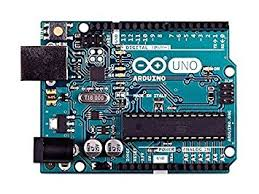
\includegraphics[width=10cm]{arduinopres}
\caption{Arduino Uno Microcontroller Board}
\end{figure}

An Arduino program was written and uploaded to the microcontroller board to handle the measurement and readout of data.  It is programmed to record values of the date and time as well as values of temperature and humidity for each sensor.  A measurement of all these properties happens every fifteen seconds.  The numerical data for each of the aforementioned parameters is recorded in a single line with the values separated by commas.

\subsection{Raspberry Pi 3B}

The Arduino Uno board is connected via a USB cable and serial programming (described in the next section) to a Raspberry Pi 3.  As can be discerned from the name, the utmost foundation of the PhysPi environmental monitoring system is the Raspberry Pi so it is obviously necessary to detail the operation of this device as it pertains to this project.

The Raspberry Pi 3 is a small, single-board computer developed for the purpose of teaching young people computer science for a financial cost significantly less than that of a full computer.  It features a Broadcom system on a chip that involves an integrated ARM compatible central processing unit and an on-chip graphics processing unit.  The 3B model, which is the one used in the PhysPi, was released in February 2016 and features a 64 bit quad core processor and has onboard Wifi, Bluetooth and USB boot capabilities. 

The Raspberry Pi 3B employs a NOOBS operating system, the usage of which is described in more detail in subsequent sections that is loaded from a Micro SD card.  For usage it requires a 2.1A micro USB power supply; without this power supply the system is not functional. The Raspberry Pi 3B has 16GB of RAM, 40 pin extended GPIO, four USB2 ports, a full size HDMI port and a micro SD port.  Other capabilities offered by the Raspberry Pi 3B that aren't utilized in this project include a CSI camera port for connecting a special Raspberry Pi camera as well as a DSI display port for connecting the Raspberry Pi to a touchscreen display.  For much of the development of this project a wired mouse, keyboard and monitor were connected to the Raspberry Pi, but this is not the exact setup being used experimentally as is discussed in Chapter 4.4.

\section{PhysPi System Software}

The development of the PhysPi software occurred across several platforms and involved programming in seven different languages (Arduino, Python, Gnuplot, MySQL, HTML, PHP and Bash).  This section will outline how these different tools came together to program the PhysPi.  It should be noted that the system is "started" when a bash script called run.sh is executed in the terminal.  This script is programmed with the proper timing and necessary paramters to run the programs that are about to be discussion in harmony with each other.

\subsection{MySQL Database}

A MySQL database was created and written on the Raspberry Pi for the purpose of data storage in this project.  MySQL is an open-source relational database management system that is often useful for storing large amounts of numerical data such as that collected by the PhysPi.  In this database (which follows the parameters listed in Appendix A) there exists a MySQL table created for this purpose with columns denoting the date and time as well as temperature and humidity values for each of the two sensors.

Through a python program that runs on the Raspberry Pi, the numerical values for each of these fields are identified based on the comma that, as mentioned previously, separates the different values.  These values are then dumped into the table in the MySQL table where they will be stored indefinitely.  This recorded data can be retrieved for later analysis or can be used for the two subsequent applications of the PhysPi.

\subsection{PhysPi Webpage}

Through programming in HTML and PHP, a webpage hosted on the Rapsberry Pi localhost was created to display the recorded data from the MySQL database in user-friendly plots and tables.  As is shown in Figure 4.3, the webpage consists of a title and heading, a table containing values of date, time, temperature and humidity for each sensor.  The webpage also displays a plot of the temperature and humidity data over time for each sensor.  As will be discussed in the next subsection, the data that is displayed in the table and plots is the last hours' worth of data.  The webpage itself refreshes every minute to provide the most current data; this is performed by the bash script mentioned previously.

\begin{figure}[h]
\centering
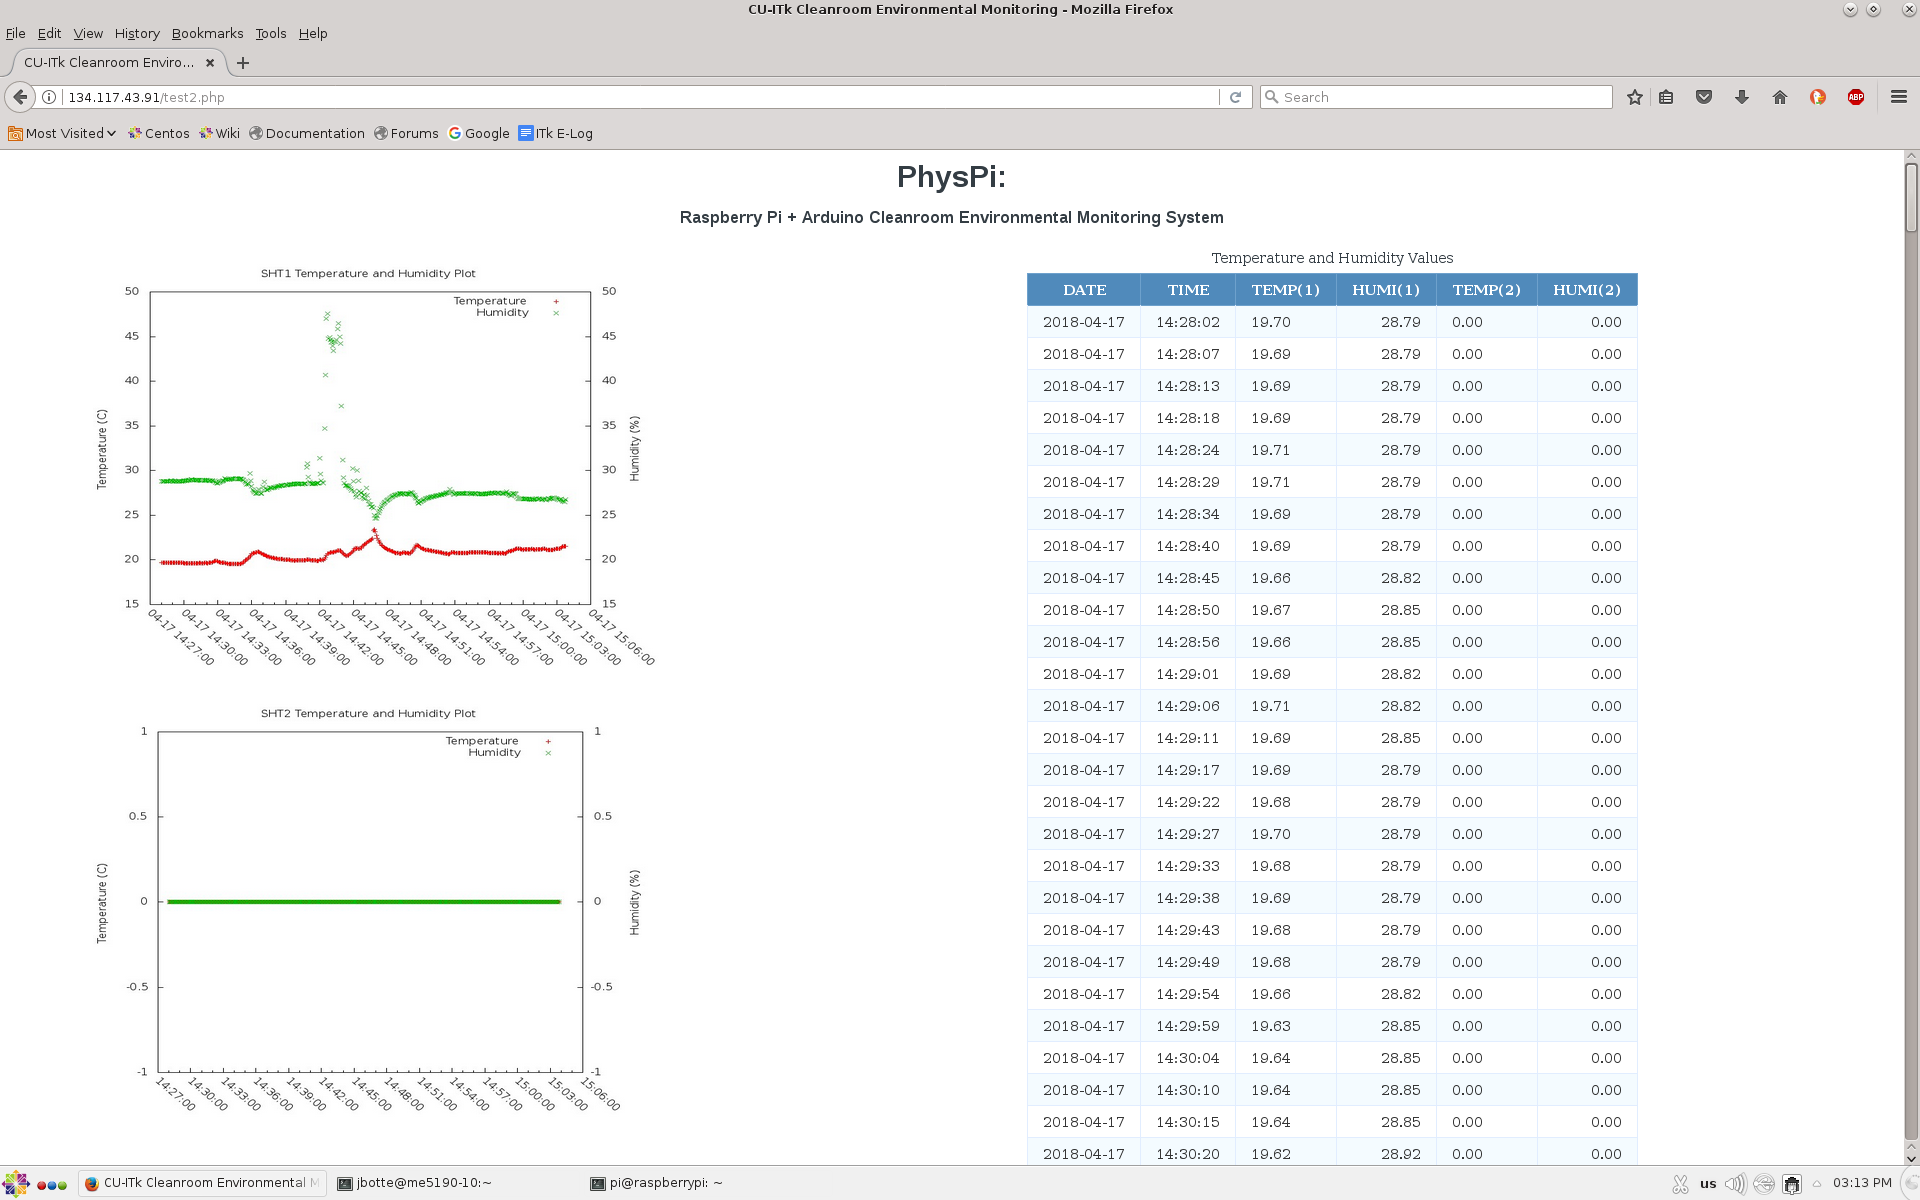
\includegraphics[width=\textwidth]{webpageprs}
\caption{PhysPi Webpage showing data from April 17th 2018}
\end{figure}

\subsection{Data Logging: Table and Graphs}

On the webpage there is an HTML table containing the values of temperature and humidity as well as the time for each sensor for each measurement taken.  This is dynamically updated and populated using PHP and HTML and refreshes automatically every 90 seconds with the past hours' worth of data as queried from the MySQL table using HTML code.  An example of this table populated with data from April 17th 2018 is shown on the right side of Figure 4.3.

Additionally, an important and likely most useful aspect of the PhysPi webpages are the plots of temperature and humidity versus time for each of the two sensors.  These plots are created using Gnuplot.  The bash script queries the past hours' worth of data from the MySQL table and the Gnuplot program reads in each row of the table individually.  It then plots the latter data columns (those being temperature and humdiity) against the data column containing values for time for each sensor.  Through the bash script, the plots update with the past hours' worth of data every minute.  An example plot for data from one of the SHT's is shown in Figure 4.4.  The y-axes of the plots are scaled automatically with the variation of data present, so a run with less variation in temperature and humidity than that what is seen in Figure 4.4 would have a much smaller y-axis and the points would be more well defined and visible.

\begin{figure}[h]
\centering
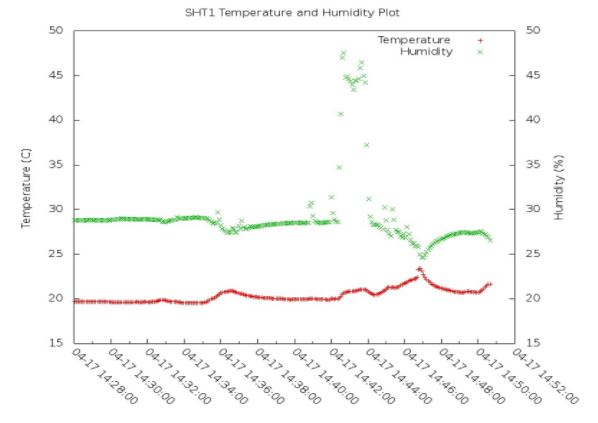
\includegraphics[width=10cm]{sht1rep}
\caption{Example Plot of Temperature and Humidity Data over Time}
\end{figure}

\section{PhysPi in the Cleanroom}

The integration of the PhysPi into the cleanroom was strategically planned in order to achieve optimal results from the system.  These plans are detailed in this section.

\subsection{Location and Physical Parameters}

As the cleanroom continues to be periodically reorganized for optimization of the various physics experiments as well as those performed by the DOE, it is likely that the PhysPi will be moved around by members of the team in order to best monitor the environmental conditions around where the strip sensors are being probed and tested.  Currently the PhysPi has been installed on the desk near the entrance to the clean room near where the cleanroom laptop and various cables are located.  Once we are able to run a longer ethernet cable from where the port is behind this desk and along the wall to the probestation, the PhysPi will be moved from the desk to near the probestation.

\subsection{Accessing the System and Webpage}

As the Raspberry Pi is technically a full computer, one normally hooks the Raspberry Pi up to a desktop monitor via a VGA or HDMI cable as well as making USB connections to a mouse and keyboard.  This is the manner by which all of the development for this project was performed.  However, in order to avoid tracking dust and other contaminants into the cleanroom with such excess hardware, the system is currently being accessed via a remote desktop connection on the cleanroom laptop.  This allows the laptop to view the entirety of the system stored on the Raspberry Pi without the need for a separate monitor, keyboard and mouse.  The bash script to start everything is run from the SSH terminal connection to the Raspberry Pi on the cleanroom laptop.

Additionally, any computer which is connected to Carleton's wifi can access the webpage from anywhere in the general vicinity of the cleanroom.  This is because such a computer will be connected to the same network as the Raspberry Pi and so the webpage is accessible by typing localhost/test2.php into the browser of the computer.  This will allow for faster access to the environmental conditions and will come in handy when the cleanroom is occuppied for other reasons but this data is needed for ITk.


\chapter{Conclusions}

The PhysPi was inducted into the cleanroom at ME5191 on April 17th 2018 and remains there at the time of this report.  Thus far it has proven useful in determining specific causes of rapid or inexplicable changes in the temperature and humidity of the room.  At the time of this work the second SHT75 sensor being used is experiencing electrical failure which has yet to be resolved.  This is expected to be a simple fix and likely will employ a new sensor.

\section{Current Results and Discussion of Relative Humidity}

Several plots of temperature and humidity data over time in the cleanroom including the one shown in Figure 4.4 from the day of the PhysPi's induction into the cleanroom.  This is not a truly accurate plot of the environmental conditions at that time as myself and another team member purposely held the sensors in such a way that variety would be produced in the data.  This was done for the purpose of ensuring that everything was working properly but has also been the source of interesting discussion regarding the exact definitions of the parameters being measured by the PhysPi.

As was shown in Figure 4.4, the humidity of the air appears to experience a drop whenever the temperature presents an increase. However, it is also shown that the humidity spikes absent of the temperature on occaision.  Fundamental physics suggest that these affects are not possible as the laws of thermodynamics dictate that temperature and humidity increase and decrease proportionally to each other.  This affect can be explained by the fact that the PhysPi measures the relative humidity of the air rather than the absolute humidity.  If it were to measure the absolute humidity then the aforementioned proportionality would be observed.  However, an increase in temeprature actually will cause a decrease in the relative humidity in the air as is observed in Figure 4.4.  The relative humidity of the air is defined by Equation 5.1: 

\begin{equation}
H_{rel} = \frac{\rho_{abs}}{\rho_{sat}}
\end{equation}

Here, \textit{H\textsubscript{rel}} is the relative humidity being measured, $\rho$\textsubscript{abs} is the absolute density of water vapour in the air and $\rho$\textsubscript{sat} is the saturated vapour density.  This saturated vapour density is taken to essentially be the maximum amount of water vapour that can be in a given volume of air.  When the temperature is increased but the amount of water molecules actually in the air remains relatively constant, this maximum vapour density will increase as the water molecules are moving more quickly and have more energy.  This means that the ratio in Equation 5.1 will decrease, which is what causes the drop in relative humidity proportional to an increase in the temperature that is shown in Figure 4.4.

However, if more water molecules are added to the air around the sensor then both the absolute and saturated vapour densities will increase, which causes the ratio in Equation 5.1 to increase.  This explains the large jump in the relative humidity also shown in Figure 4.4 that occurs absent of any small temperature change.

\section{Future Work and Extensions}

The PhysPi holds the potential for a large amount of further development in the future.  The ideas described in this section are what I see as being logical and helpful extensions of the PhysPi.

Currently the webpage displays only plots of the temperature and humidity over time in addition to the raw data table.  This analysis of the data should be expanded as the team sees fit; in the future it may be necessary to obtain a more detailed statistical analysis of the data recorded to observe trends and investigate the possible causes of any trends that arise.

As the CU-ITk already utilizes more than two SHT75 sensors at once for other testing, it would be productive to at some point expand the PhysPi system to employ more than two sensors.  This would allow for a more accurate assessment of the overall temperature and humidity of the cleanroom as it would mean measuring these parameters at more than two locations within the room.  Specifically, it would likely be useful to deploy six or eight sensors in a circular formation around the probestation for extremely accurate environmental monitoring of the probestation.  

At the present time it is hypothesized that the PhysPi will work in it's current state for at least several months to a year, but eventually the shear amount of information being stored in the MySQL database will be enough to overpower the Raspberry Pi.  Before this occurs, the database should be transferred to one that is stored on the cleanroom laptop rather than on the Raspberry Pi itself.  As long as the Raspberry Pi and the cleanroom laptop are connected to the same network this is a relatively straightforward and simple procedure that can be carried out by future students.

Open physics questions that have yet to be solved at the time of this work include the fluctuation of various parameters measured by the PhysPi and if these fluctuations have a higher dependence on the relative humidity of the air present (which is what the PhysPi measures) or if the higher dependence is on the absolute humidity percentage of the air.  This concept relates to proton absorbtion of several aspects of the system and will require several trials of the PhysPi to determine with a high-level of accuracy.

\appendix
%\appendixpage
%\addappheadtotoc
\chapter{PhysPi Datasheet} 

This datasheet will outline any and all parameters and information necessary for the accurate operation and usage of the PhysPi following my graduation and departure from Carleton University and Ottawa.  It is intended to be kept in the cleanroom near where the PhysPi is stationed for easy access.

\begin{itemize}
\item Raspberry Pi username (non-root): pi
\item Raspberry Pi password (non-root): raspberry
\item MySQL username (non-root): cuitkuser
\item MySQL password (non-root): cuitk
\item MySQL Database used: 2sht
\item Physics Department IP Address: 134.117.23.229
\item Department of Electronics IP Address: 134.117.43.91
\item SHT1 temperature port: 10
\item SHT1 humidity port: 12
\item SHT2 temperature port: 8
\item SHT2 humidity port: 4
\end{itemize}

To run the programs necessary to complete all PhysPi tasks, SSH into the Pi (**using root user**) from the cleanroom laptop and type "./run.sh" to execute the master program, then leave it running.  If it is stopped for any reason be sure to rerun it.  The DOE IP address is the one corresponding to the Pi as it is setup right now in the cleanroom.  The one for the Physics Department will likely only need to be used for maintenence that must occur outisde the cleanroom.

\begin{thebibliography}{9}

\bibitem{robthesis}
R. Hunter,
\textit{Development and Evaluation of Novel, Large-Area, Radiation Hard Silicon Microstrip Sensors for the ATLAS ITk Experiment at the HL-LHC}
\\MSc Thesis, Deparment of Physics, Carleton University, 2017.

\bibitem{koffasnotes}
T. Koffas,
\textit{Fermi Energy and Pauli's Principle: Gravitational Collapse of Dead Stars}
\\PHYS 3606 Lecture Notes, Department of Physics, Carleton University, 2016.

\bibitem{hyperphysics}
R. Nave,
\textit{Fermi Level and Fermi Function}
\\\texttt{http://hyperphysics.phy-astr.gsu.edu/hbase/Solids/Fermi.html}

\bibitem{atlasspecs}
ATLAS
\textit{Technical Specification - Supply of Silicon Microstrip Sensors of ATLAS12EC Specification}
\\ATLAS Upgrade Strip Sensor Collaboration, 2015.

\bibitem{zegh}
B. Zeghbroeck,
\textit{The P-N Junction Capacitance}
\\\texttt{https://ecee.colorado.edu/~bart/book/pncap.htm}

\bibitem{cern}
CERN,
\textit{The Large Hadron Collider}
\texttt{https://home.cern/topics/large-hadron-collider}

\bibitem{rel}
R. Nave,
\textit{Relative Humidity}
\texttt{http://hyperphysics.phy-astr.gsu.edu/hbase/Kinetic/relhum.html}



\end{thebibliography}


\end{document}